% This must be in the first 5 lines to tell arXiv to use pdfLaTeX, which is strongly recommended.
\pdfoutput=1
% In particular, the hyperref package requires pdfLaTeX in order to break URLs across lines.

\documentclass[11pt]{article}

% Remove the "review" option to generate the final version.
\usepackage{ACL2023}

% This is not strictly necessary, and may be commented out.
% However, it will improve the layout of the manuscript,
% and will typically save some space.
\usepackage{microtype}

% This is also not strictly necessary, and may be commented out.
% However, it will improve the aesthetics of text in
% the typewriter font.
\usepackage{inconsolata}

\usepackage[utf8]{inputenc} % allow utf-8 input
\usepackage[T1]{fontenc}    % use 8-bit T1 fonts
\usepackage{hyperref}       % hyperlinks
\usepackage{url}            % simple URL typesetting
\usepackage{booktabs}       % professional-quality tables
\usepackage{amsfonts}       % blackboard math symbols
\usepackage{nicefrac}       % compact symbols for 1/2, etc.
\usepackage{microtype}      % microtypography
\usepackage{xcolor}         % colors

% --- Copied: begin
% Standard package includes
\usepackage{times}
\usepackage{latexsym}

\usepackage{graphicx}
\usepackage{subfigure}
\usepackage{booktabs} % for professional tables
\usepackage{lipsum}
\usepackage{amsmath}
\usepackage{amssymb, amsthm, latexsym}
\usepackage{multirow}

\usepackage{nicefrac}

% \usepackage{minted}
% To submit on arxiv, comment the line above and follow this: https://github.com/gpoore/minted/issues/113#issuecomment-888045507
% \usepackage[finalizecache,cachedir=.]{minted}
\usepackage[frozencache,cachedir=.]{minted}

\newminted{python}{%
    fontsize=\fontsize{8.25pt}{8.25pt}\selectfont,
    % options to customize output of pythoncode
}
% --- Copied: end


% If the title and author information does not fit in the area allocated, uncomment the following
%
%\setlength\titlebox{<dim>}
%
% and set <dim> to something 5cm or larger.

\title{\textsc{Petals}: Collaborative Inference and Fine-tuning of Large Models}

% Author information can be set in various styles:
% For several authors from the same institution:
% \author{Author 1 \and ... \and Author n \\
%         Address line \\ ... \\ Address line}
% if the names do not fit well on one line use
%         Author 1 \\ {\bf Author 2} \\ ... \\ {\bf Author n} \\
% For authors from different institutions:
% \author{Author 1 \\ Address line \\  ... \\ Address line
%         \And  ... \And
%         Author n \\ Address line \\ ... \\ Address line}
% To start a seperate ``row'' of authors use \AND, as in
% \author{Author 1 \\ Address line \\  ... \\ Address line
%         \AND
%         Author 2 \\ Address line \\ ... \\ Address line \And
%         Author 3 \\ Address line \\ ... \\ Address line}

\author{
  Alexander Borzunov\thanks{\ \ Equal contribution. Correspondence to:\newline \texttt{borzunov.alexander@gmail.com}}\\
  HSE University, Yandex \\\And
  Dmitry Baranchuk$^*$ \\
  Yandex \\\And
  Tim Dettmers$^*$ \\
  University of Washington\\\AND
  Max Ryabinin$^*$ \\
  HSE University, Yandex \\\And
  Younes Belkada$^*$ \\
  Hugging Face, ENS Paris-Saclay \\\And
  Artem Chumachenko \\
  Yandex \\\AND
  Pavel Samygin \\
  Yandex School of Data Analysis \\\And
  Colin Raffel \\
  Hugging Face
}

\begin{document}
\maketitle
\begin{abstract}
Many NLP tasks benefit from using large language models (LLMs) that often have more than 100 billion parameters. With the release of BLOOM-176B and OPT-175B, everyone can download pretrained models of this scale. Still, using these models requires high-end hardware unavailable to many researchers. In some cases, LLMs can be used more affordably via RAM offloading or hosted APIs. However, these techniques have innate limitations: offloading is too slow for interactive inference, while APIs are not flexible enough for research that requires access to weights, attention or logits. In this work, we propose \textsc{Petals}\footnote{\textsc{Petals} source code and documentation are available at \texttt{\href{https://petals.ml}{https://petals.ml}}} --- a~system for inference and fine-tuning of large models collaboratively by joining the resources of multiple parties. We demonstrate that this strategy outperforms offloading for very large models, running inference of BLOOM-176B on consumer GPUs with $\approx$~1 step per second, which is enough for many interactive LLM applications. Unlike most inference APIs, \textsc{Petals} also natively exposes hidden states of served models, allowing to train and share custom model extensions based on efficient fine-tuning methods.
\end{abstract}

\section{Introduction}\label{sect:intro}

Many recent influential discoveries in deep learning were enabled by the trend of scaling model and dataset size.
Over the last decade, computer vision has grown from training models with 60 million parameters~\cite{alexnet} on 1.3 million images~\cite{imagenet_cvpr09} to 15 times more parameters~\cite{Kolesnikov2020BigT} and 200 times more training data~\cite{jft-300m}. In natural language processing, the state-of-the-art language models~\cite{gpt3} with 175 billion parameters are trained on over 570GB of texts, and even this does not saturate the model quality~\cite{kaplan2020scaling}.
Training these large models can take years even with a top-of-the-line GPU server~\cite{gpt3costlambda}. As a result, researchers and practitioners often have to run distributed training with multiple machines~\cite{mlperf}.

The dominant approach to distributed deep learning is data-parallel training~\cite{valiant1990bridging}, where each worker processes a fraction of the training batch and then exchanges its gradients with peers. If done naïvely, the gradient exchange step can overload the network as the number of workers increases. To combat this issue, modern distributed training algorithms take advantage of communication-efficient protocols, such as all-reduce~\cite{bandwidth_optimal_allreduce}. These protocols 
allow workers to collectively compute the global average gradient with a constant communication overhead, regardless of the total number of peers.

However, this efficiency makes the protocols more fragile: if any single participant fails or takes too long to process its batch, all other nodes are stalled.
Therefore, scaling all-reduce protocols beyond a couple of servers requires specialized infrastructure with dedicated ultra-high bandwidth networking~\cite{mlperf}.
This kind of infrastructure is notoriously expensive compared to regular
GPU servers or preemptible cloud VMs (see Appendix~\ref{sect:cloud_costs} for details).

Hence, it is tempting to consider distributed training on cheap unreliable instances as a cost-efficient alternative. A similar scenario arises in federated learning~\cite{mcmahan2017communication}, where a single model is trained on heterogeneous devices due to privacy concerns.
In both scenarios, workers use a shared network, where both latency and bandwidth can vary drastically due to interference from other users~\cite{variability_azure}\nocite{variability_aws}. Furthermore, compute nodes are also subject to failure (or preemption) caused by factors beyond the protocol's control.

Running large-scale distributed training in these circumstances requires fault- and latency-tolerant algorithms~\cite{lian2017can,sgpush}. Most of these algorithms replace all-reduce averaging with \textbf{gossip}: each participant periodically downloads the latest parameters from their neighbors in a sparsely connected communication graph and averages the results. The updates gradually propagate through the graph over multiple rounds of averaging.
However, the communication required to perform gossip grows linearly with the number of neighbors. Hence, when scaling to hundreds of peers, decentralized SGD has to keep the communication graph sparse, slowing down the convergence.

In this work, we propose an alternative approach. Instead of relying on a predefined communication graph, participants dynamically organize themselves into groups using a fully decentralized matchmaking algorithm called \textbf{Moshpit All-Reduce}. This strategy allows us to use communication-efficient all-reduce protocols that significantly reduce the network load compared to gossip-based averaging, while still being able to operate in unreliable hardware and network conditions.

Our contributions can be summarized as follows:
\begin{itemize}
    \item We propose {\bf Moshpit All-Reduce} --- a novel decentralized averaging protocol for large-scale training with unreliable communication-constrained devices. According to our analysis, this method has exponential convergence rate independent of network topology and size.
    \item Armed with this averaging protocol, we develop {\bf Moshpit SGD} for distributed optimization. We derive convergence rates for this algorithm and establish its equivalence to Centralized (Local) SGD in terms of iteration complexity under realistic assumptions.
    \item Our experiments demonstrate that Moshpit All-Reduce is significantly more efficient under network latency in realistic conditions. In particular, we train ResNet-50 on ImageNet to 75\% accuracy 1.3 times faster than existing decentralized training algorithms and pretrain ALBERT-large 1.5 times faster on preemptible cloud VMs.\footnote{Implementation and code of experiments are at \href{https://github.com/yandex-research/moshpit-sgd}{\texttt{github.com/yandex-research/moshpit-sgd}}.}
\end{itemize}

\section{Design and use cases}

Practical usage of large language models can be broadly divided into two main scenarios: inference and parameter-efficient adaptation to downstream tasks. In this section, we outline the design of \textsc{Petals}, showing how it handles both scenarios and also allows easily sharing trained adapters between the users of the system.

\subsection{Inference of billion-scale models}\label{sect:design_inference}

When generating tokens, a client stores the model's token embeddings (which typically comprise a small fraction of the total parameter count and can fit in RAM in most modern laptops, servers, and workstations) locally and relies on servers to run Transformer blocks. Each server holds several \textit{consecutive} blocks, the number of which depends on the server's available GPU memory.
Before each inference session, the client finds a chain of servers that collectively hold all model layers.

Once the chain is formed, the client uses the local embedding layer to look up embedding vectors for prefix tokens, then sends those vectors to servers and receives new representations. Once the client obtains the outputs of the final block, it computes next token probabilities and repeats this process.
%\footnote{Most LLMs, including BLOOM, reuse the embedding matrix to compute next token probabilities}

While the session is active, servers store attention keys and values from past client inputs and use them for subsequent inference steps. Clients also store past inputs to each server so that if any server fails or goes offline, another one can quickly take its place. The procedure for finding servers and recovering from failures is detailed in Section~\ref{sect:networking}.

\paragraph{Client-side API.} To generate tokens with \textsc{Petals}, one first creates an \textit{inference session}. An inference session iteratively takes inputs as PyTorch tensors, runs them through all Transformer blocks and returns final representations as PyTorch tensors. Under the hood, sessions form server chains, hold cache, and recover from server failures in a way that is transparent to the user. An example of using an inference session is shown in Figure~\ref{fig:infernce_snippet}.

% Optionally, clients can send the same embeddings to multiple servers holding the same block. This allows client to verify the correctness of their inference by cross-checking clients. This can also be used to achieve consistently low latency if some servers experience delays.

\begin{figure}[tb]
\small
\begin{pythoncode}
# Initialize distributed BLOOM model
model = DistributedBloomForCausalLM \
    .from_pretrained("bigscience/bloom-petals")
input_ids = tokenizer(prefix_text)

with model.inference_session() as session:
    # Session maintains a set of servers that
    # store attention KV from previous steps
    for _ in range(sequence_length):
        # Compute the word embeddings locally
        hid = model.word_embeddings(input_ids)
        # Run distributed Transformer blocks,
        # store attention KV for future steps
        hid = session.step(hid)
        # Sample the next token locally
        probs = model.lm_head(hid)
        input_ids = sample_next_token(probs)
\end{pythoncode}
    \vspace{-5pt}
    \caption{A basic PyTorch code snippet for generation with a distributed BLOOM-176B model.}
    \label{fig:infernce_snippet}
    \vspace{-10pt}
\end{figure}

\paragraph{System requirements.} For BLOOM-176B inference, clients need at least 12 GB RAM, most of which is used to store 3.6B embedding parameters. We recommend at least 25 Mbit/s bidirectional bandwidth to avoid bottlenecks in network transfers. Simple greedy inference can use any CPU that runs PyTorch, but more advanced algorithms (e.g., beam search) may require a GPU.

In turn, servers need at least 16 GB of CPU RAM, 100 Mbit/s bandwidth and a GPU with at least 8~GB of memory.

\paragraph{Chat application.} We also provide an example application that lets users chat with LLMs in a messenger-like user interface (see Figure~\ref{fig:chat_app}). The application supports BLOOM-176B and BLOOMZ-176B, a version of BLOOM fine-tuned to better perform in the zero-shot regime~\cite{bloomz}. The application is comprised of the \textit{frontend} and the \textit{backend}.
The frontend is a web page that allows users to communicate with the model by prompting it with text and receiving the generated output.
The backend is a Flask web server that uses the \textsc{Petals} client to run inference over the swarm. It accepts requests via HTTP or Websocket protocols, so anyone can develop their own applications using our backend for inference.

%figure moved to the other column

\subsection{Training for downstream tasks}\label{sect:design_training}

While LLMs achieve high quality on many problems with simple prompt engineering~\citep{gpt3}, they often need training to achieve the best results. Traditionally, this is done by fine-tuning all model parameters on the downstream task.
%Adapting a single large pre-trained language model to multiple tasks and domains is a de facto standard for many downstream generation and natural language understanding (NLU) applications. \textit{Full fine-tuning}, which updates all model parameters, often demonstrates state-of-the-art performance.
However, for very large models, this strategy becomes impractical due to hardware requirements. For example, fine-tuning BLOOM-176B with Adam would require almost 3~TB of GPU memory to store model, gradients, and optimizer states.

To combat this issue, the NLP community has developed \textit{parameter-efficient fine-tuning} methods that keep most of the pretrained model intact. Some of them~\citep{sung2021training,guo2021parameter} choose a subset of existing parameters, others~\citep{hu2021lora, houlsby2019parameter, ptune-liu, ptune-lester, ptune-v2, tfew} augment the model with extra trainable weights.

Despite their lower memory requirements, parameter-efficient approaches are often competitive with full model fine-tuning \citep{hu2021lora,ptune-v2,yong_adapting} and even outperform it in low-data regimes~\citep{2205.05638}. Another appealing property of these approaches for our use-case is that they allow rapidly switching a pretrained LLM between different uses.

%note: the paragraph below was commented due to spacing cosntraints
% -- It can be reintroduced later if we have some room to spare
% Overall, efficient adaptation of large language models is an essential direction that makes them appealing for real-world applications. Thus, in our demonstration, we put significant effort into providing \textbf{accessible}, \textbf{user-friendly}, \textbf{reliable} and \textbf{efficient} service for BLOOM-176B adaptation.

\begin{figure}[tb]
    \centering
    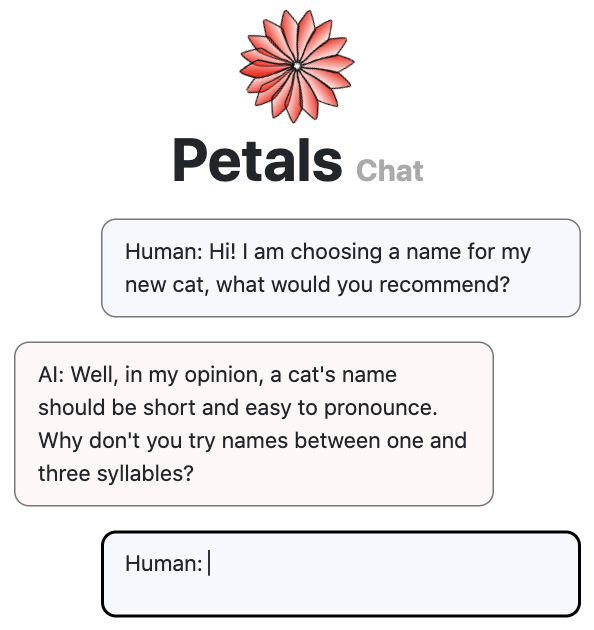
\includegraphics[width=0.9\linewidth]{resources/chat_app.png}
    % \vspace{-5pt}
    \caption{A chat application that runs BLOOM-176B or BLOOMZ-176B over the \textsc{Petals} swarm, available at \texttt{\href{https://chat.petals.ml}{https://chat.petals.ml}}}
    \label{fig:chat_app}
    \vspace{-10pt}
\end{figure}

\paragraph{Distributed fine-tuning.} The core principle of fine-tuning in a distributed network is that clients ``own'' trained parameters while servers host original pretrained layers. Servers can run backpropagation through their layers and return gradients with respect to activations, but they \textit{do not update the server-side parameters}. Thus, clients can simultaneously run different training tasks on the same set of servers without interfering with one another.

% \begin{figure}[tb]
%     \centering
%     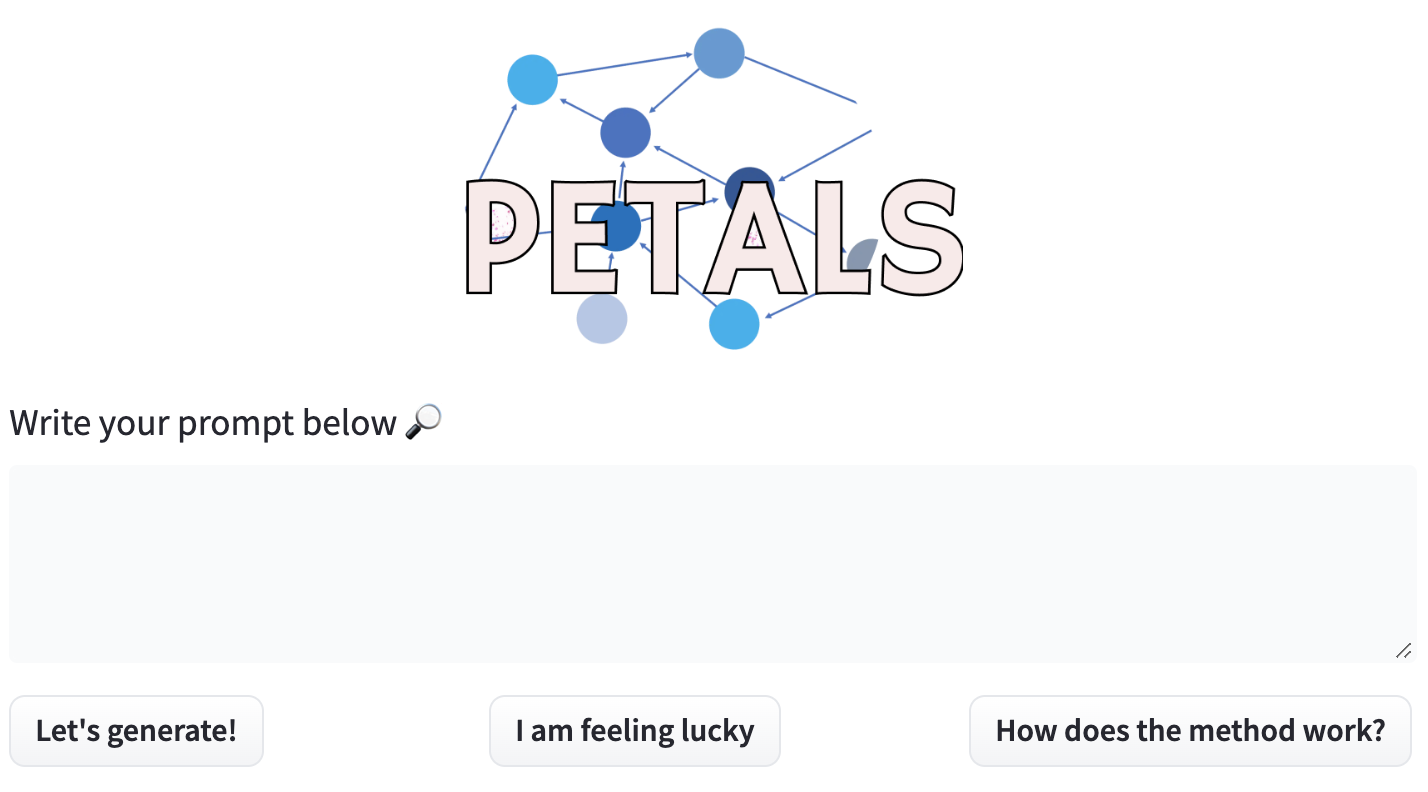
\includegraphics[width=0.7 \linewidth]{resources/GUI.png}
%     \caption{A prototype of the user interface for inference with \textsc{Petals}.}
%     \label{fig:infernce_ui}
%     \vspace{-5pt}
% \end{figure}

% In more detail, each user locally stores a few trainable parameters, e.g, tunable prompts or adapters. At each training iteration, a client sends his inputs and parameters to the remote model. A sequence of servers perform forward and backward operations and send the gradients w.r.t. client's parameters back. The client receives the gradients and locally updates the parameters. 

To illustrate this principle, we first review an example of soft prompt-tuning for text classification and then generalize it to other methods and tasks.
Similarly to Section~\ref{sect:design_inference}, clients store the embedding layers locally and rely on servers to compute the activations of Transformer blocks. In this fine-tuning scenario, a client needs to store trainable soft prompts (task-specific input embeddings) and a linear classification head. 

For each training batch, the client routes its data through a chain of remote servers to compute sentence representations, then obtains predictions with the classifier head and computes the cross-entropy loss.
%NOTE: this intentionally avoids talking about load balancing and fault tolerance
During backpropagation, the client runs its data through the same chain of servers in reverse order to compute gradients for the learned prompt vectors. Having obtained those gradients, the client can use a regular PyTorch optimizer to update the parameters of both the head and the prompts, then proceed to the next minibatch.

\paragraph{User interface.} To allow users greater flexibility in their training workloads, we made distributed backpropagation module compatible with the PyTorch Autograd engine. Like in the inference stage, this module handles fault tolerance and load balancing transparently to the user while allowing them to access intermediate activations and insert custom PyTorch modules. Figure~\ref{fig:training_snippet} shows an example training code snippet.

%provide state-of-the-art parameter-efficient fine-tuning methods, which do not update the initial model weights\citep{p-tune. p-tune-v2, lora}. 
This interface can also support other popular parameter-efficient fine-tuning algorithms, such as LoRA~\citep{hu2021lora} or prefix tuning~\citep{li-liang-2021-prefix}. Finally, users can insert custom local modules after some of the  existing blocks, which could allow use-cases like retrieval-augmented generation~\citep{retro,rag}.% or sparse Mixture-of-Experts layers~\citep{Lepikhin2020GShardSG,switch,base}.

\begin{figure}[tb]
\small
\begin{pythoncode}
# Use distributed BLOOM with soft prompts
model = AutoModelForSequenceClassification \
    .from_pretrained(
        "bigscience/bloom-petals",
        tuning_mode="ptune", pre_seq_len=5)
# Define optimizer for prompts and linear head
opt = torch.optim.AdamW(model.parameters())

for input_ids, labels in data_loader:
    # Forward pass with local & remote layers
    out = model.forward(input_ids)
    loss = cross_entropy(out.logits, labels)

    # Distributed backward w.r.t. local params
    loss.backward() # Compute prompts.grad
    opt.step() # Update local params only
    opt.zero_grad()
\end{pythoncode}
\vspace{-5pt}
\caption{A basic PyTorch code of soft prompt tuning for sequence classification with \textsc{Petals}.}
\label{fig:training_snippet}
\vspace{-10pt}
\end{figure}


% \textbf{System requirements.} The minimal training script for soft prompt-tuning requires 16GB RAM and benefits from high network bandwidth.
% Similarly to Section~\ref{sect:design_inference}, nearly half of all memory is used on pre-trained embeddings, while the few trainable parameters have negligible memory footprint. Intermediate activations also use little memory due to the use of gradient checkpointing~\citep{gradient_checkpointing_autograd,gradient_checkpointing_dl}. Naturally, workloads with more trainable parameters will require additional memory and often benefit from having a local GPU.


% This training procedure makes the system \textbf{cheap} and \textbf{accessible} since the users can perform the model adaptation on their laptops, desktops or Colab notebooks. The minimum hardware requirements are only <TODO> GBs of RAM and $100$ Mbps network speed.

% Moreover, since the adaptation methods do not update the parameters of the pre-trained model, multiple users can solve their individual tasks at the same time. In addition, researchers and developers can readily incorporate their custom PEFT methods.

% Importantly, all distributed details are hidden inside standard PyTorch methods. Thus, users only have to run a simple PyTorch training loop to adapt the BLOOM-176B to their tasks. We provide an example of the the training code in Figure~\ref{figure:training_snippet}. During the demonstration, users will be able to give it a try and solve sequence classification and <TODO: some generative task> on public datasets.

% \begin{itemize}
%     \item \textbf{Accessible:} Each user can adapt the model on his desktop / laptop / colab having only <TODO> GBs of RAM and $100$ Mbps network speed; 
%     \item \textbf{Flexible:} 
%         \begin{itemize}
%             \item Multiple users can solve their individual tasks independently at the same time;
%             \item Users can customize or incorporate their own adaptation methods;
%         \end{itemize}
%     \item \textbf{High-quality:} Suggest state-of-the-art parameter-efficient model adaptation methods;
%     \item \textbf{User-friendly:} High-level API for regular users and standard PyTorch training code for developers and researchers;
% \end{itemize}

% \textbf{Parameter-efficient fine-tuning.} Exists. Describe prompt-tuning, adapters, yield from 2205.05638. Cite relevant papers.

% Users can hold their prompts / adapters locally with limited RAM. Two users can simultaneously train two prompts / adapters without interfering with one another. Servers only hold ``permanent'' bits of the model.

% \textbf{Demo part with prompt tuning:} explain what we provide. Client stores only embeddings and learned prompts -> prompt-tuning can be done in colab / on a commodity desktop. Code is similar to training locally.


% \textbf{Flexible interface for researchers.} Explain how researchers can insert their own custom modules for RAG / RETRO / MoE / PKM in the middle of the model. Supports torch autograd.



% FILLER TEXT TO ACCOUNT FOR MISSING CONTENT \lipsum[5]


\subsection{Sharing and reusing trained modules}
\label{sect:design_ecosystem}

Although most fine-tuned extensions for pretrained models can be easily shared as-is, simplifying the workflow for sharing these extensions enables users to more easily adapt the model to their target scenario. Indeed, existing model hubs~\citep{wolf-etal-2020-transformers, tfhub, torchhub} have gained immense popularity due to many supported models and ease of use, especially when vetting different pretrained models for a given problem. One particularly relevant project is AdapterHub~\citep{adapterhub}, a repository of trained adapters accompanied by a library with implementations of different adaptation methods. While \textsc{Petals} does not depend on AdapterHub, it is possible to leverage this library for training adapters in the distributed setting.
%We were also inspired by it when designing our streamlined solution for adapter sharing.
Instead, we support sharing modules trained by users via the Hugging Face Hub (also used as a backend by AdapterHub). Its infrastructure and the corresponding open source library simplify the learning process for users already familiar with the ecosystem. Because the primary navigation mechanism on the Hugging Face Hub are tags that have been applied to uploaded modules, a user only needs to the task it was trained on and the model upon which the adapter was built. Uploading the weights and the code of the fine-tuned module is done by committing them to a Git repository.
When navigating the Hub, users can choose the most suitable adapters by filtering the list of all available modules by the required tags.
\section{Internal structure and optimizations}\label{sect:internals}


One of the primary considerations for distributed inference is its performance. It can be broken down into three main aspects: computation speed (5-year-old gaming GPU vs. new data center GPU), communication delay due to distance between nodes (intercontinental vs. local), and communication delay due to bandwidth (10 Mbit/s vs. 10 Gbit/s).

In terms of raw FLOPs, even consumer-grade GPUs like GeForce RTX 3070 could run a complete inference step of BLOOM-176B in less than a second~\citep{ga102-datasheet}. However, the GPU memory can only hold a small fraction of model layers: running na\"ively would require 44 RTX 3070 GPUs and 44 communication rounds. To make this more efficient, we use quantization to store more parameters per GPU, reducing the number of consecutive devices and communication rounds (Section~\ref{sect:inside_gpu}). On top of that, each client prioritizes nearby servers to make communication rounds faster (Section~\ref{sect:networking}).

% partially moved to 3.2
%While GPU performance differs by roughly 3-5x at most, communication time can differ by many orders of magnitude. %(local Gbit communication vs global MBit communication).
%Latency can even be unbounded in case of node failures. As such, optimizations related to latency are the most critical components for a practical distributed inference system — a single high latency communication can lead to poor inference runtime performance.

% this paragraph was moved to 3.2
% We can optimize latency through  optimizations, that is, compressing weights and hidden states, and, secondly, through graph optimizations, that is optimize the communication between users so that the total communication cost for an inference pass is on average minimal.

\subsection{Large model inference on consumer GPUs}\label{sect:inside_gpu}

% YOZH: paraphrased this sentence, moved some of the motivation to 3.0
% orginal: One of our main goals is democratization of large pretrained models. As such, our distributed inference method is designed to work well on
We assume that each server has at least 16 GB of CPU RAM, 8 GB of GPU memory. From this assumption, one of the primary considerations is to reduce the model memory footprint, so that each device can hold more Transformer blocks.% [MOVED TO Section 3.0], thus less communication between users has to be done to process all transformers blocks to complete a forward/backward pass.

For example, BLOOM has 176B parameters, which takes 352 GB of GPU memory in 16-bit precision. Thus, in the worst case, the model is distributed among 352 GB / 8 GB (per server) = 44 nodes. We can reduce both frequency and amount of data transfer in two ways.
First, we can achieve this by compressing the hidden states exchanged between nodes. Second, we can compress the weights to 8-bit precision, reducing the number of nodes required to hold all layers. For BLOOM, this changes the number of required nodes from 44 to 22, which reduces latency in half and decreases the probability of a failure.

\paragraph{Compressing communication buffers.} To send less data between subsequent pipeline stages, we use dynamic blockwise quantization \citep{dettmers2022optimizers}. We apply it to the hidden states before pipeline-parallel communication, as done in \citet{ryabinin2021swarm}. Dynamic blockwise quantization halves the bandwidth requirements without any noticeable effect on generation quality.

\paragraph{Compressing model weights.} We use 8-bit mixed matrix decomposition for matrix multiplication to quantize the weights to 8-bit precision and reduce the memory footprint compared to 16-bit weights, as suggested in \citep{dettmers2022llm}. This decomposition separates hidden states and weights into two portions: about 0.1\% of 16-bit outlier and 99.9\% of 8-bit regular values, which roughly halves the memory footprint.

% \begin{table}[tb]
% \centering
% \caption{Zero-shot accuracy for OPT-175B and BLOOM-176B with 8-bit and 16-bit weights.\nocite{eval-harness}}
% \vspace{-8px}
% \label{tbl:resutls8bit}
% % \small
% % \setlength{\tabcolsep}{2pt}
% \resizebox{\linewidth}{!}{%
% \begin{tabular}{lcccccc}\toprule
% \bf Model    &\bf Bits &\bf HellaSwag &\bf PIQA & \bf LAMBADA &\bf WinoGrande &\bf Avg  \\\midrule
% \multirow{2}{*}{OPT-175B} & 16   & 78      & 81 & 75    & 72       & 77 \\
%  & 8    & 78      & 81 & 75    & 72       & 77 \\\midrule
% \multirow{2}{*}{BLOOM}    & 16   & 73      & 79 & 67    & 70       & 73 \\
%    & 8    & 73      & 79 & 68    & 70       & 73 \\\bottomrule
% \end{tabular}%
% }
% \label{tab:quality}
% \vspace{-4pt}

% \end{table}

As shown in Table~\ref{tab:quality}, this method has little effect on LLM quality for major benchmarks.
In terms of inference time, Table~\ref{tab:throughput} demonstrates that quantization has about $5\%$ of overhead with batch size 1 (20 tokens), but becomes negligible for larger batches.

% TODO:
% \begin{itemize}
%     \item quality benchmarks v.s. original model (Tim: I need to write some CUDA kernels for the final data; initial tests indicate no ppl degradation on OPT-66B)
%     \item performance (aka speed) benchmarks v.s. original model (locally) (Younes has these completed for BLOOM)
%     \item any extra optimizations?
%     \item how to convert your own model (we have HF integration, if distribute inference is build on the HF pretrained models this should work for any model)
% \end{itemize}

\subsection{Collaborating over the Internet}\label{sect:networking}

\begin{table}[tb]
\centering
\caption{Zero-shot accuracy for OPT-175B and BLOOM-176B with 8-bit and 16-bit weights.\nocite{eval-harness}}
\vspace{-5pt}
\resizebox{\linewidth}{!}{%
\begin{tabular}{lccccc}\toprule
\textbf{Model}            & \textbf{Bits} & \textbf{HellaSwag} & \textbf{LAMBADA} & \textbf{WinoGrande} & \textbf{Avg}             \\\midrule
\multirow{2}{*}{OPT-175B} & 16            & 78.5               & 74.7             & 72.6                & 75.3                     \\
                          & 8             & 78.5               & 74.6             & 71.7                & \multicolumn{1}{r}{74.9} \\\midrule
\multirow{2}{*}{BLOOM}    & 16            & 73.0               & 67.2             & 70.1                & 70.1                     \\
                          & 8             & 72.8               & 68.1             & 70.1                & 70.3                    \\\bottomrule
\end{tabular}}
\label{tab:quality}
% \vspace{-5pt}
\end{table}

\begin{table}[tb]
% \vspace{-8px}
\centering
\caption{Generation throughput (tokens/s) for BLOOM-176B with 8-bit and 16-bit weights on 8$\times$~A100 GPUs.}
\vspace{-5pt}
\label{tbl:memory_footprint}
\resizebox{0.5\linewidth}{!}{%
\begin{tabular}{lccc}\toprule
\multirow{2}{*}{\bf Weights}& \multicolumn{3}{c}{\bf Batch size} \\\cmidrule{2-4} & \bf 1 & \bf 8 &\bf 32  \\\toprule
16-bit       & 4.18 & 31.3  & 100.6  \\
8-bit        & 3.95 & 29.4  & 95.8\\\bottomrule
\end{tabular}}
\label{tab:throughput}
\vspace{-10pt}
\end{table}

Another challenge is to provide \textit{reliable} inference and training despite nodes joining, leaving or failing at any time. To address this, \textsc{Petals} uses the \texttt{hivemind} library~\citep{hivemind} for decentralized training and custom fault-tolerant protocols for servers and clients.

% \begin{itemize}
%     \item Design constraints? (limited network bandwidth,  heterogeneous devices, hardware and network failures)
%     \item activation quantization
%     \item user doesn't want manual tuning, manual error handling, etc
%     \item latency-aware activation routing
%     \item servers determine which blocks are in most demand
%     \item servers are as stateless as possible, client stores everything needed to recover from server failure
%     \item how to convert your own model
% \end{itemize}

\paragraph{Server load balancing.} First, we ensure that servers are distributed evenly among Transformer blocks. Formally, servers maximize the total model throughput by choosing the blocks with the worst throughput and eliminating potential bottlenecks.

Each server periodically announces its active blocks to a distributed hash table~\citep{kademlia}. When a new server joins, it uses this information to identify an interval of blocks that contains most blocks with the worst throughput. This interval is always contiguous, since splitting it would harm the inference latency. Once the server has selected its layers, it measures its own throughput (both network and compute) and announces it to the distributed hash table. %(the minimum of its network and compute throughputs).

Since peers may leave or fail at any time, all nodes periodically check if launching a rebalancing procedure would significantly improve the overall throughput. If it is the case, they switch layers until the throughput becomes near-optimal. In particular, if all peers serving certain blocks suddenly leave the system, this procedure quickly redistributes the remaining resources to close the emerged gaps.

% \textbf{Efficient network communication.} During inference or training, both clients and servers send high dimensional intermediate activations or gradients through the Internet. Therefore, high network latency and limited bandwidth can significantly reduce throughput of the overall system. 

% By default, peers communicate via half-precision tensors. However, we also propose to additionally quantize them into Int8 by the recent blockwize quantization method\citep{}. This method is shown to have low error rates being computationally efficient. Thus, this approach allows us to halve the network traffic without noticeable accuracy losses and computational costs.

\paragraph{Client-side routing.} Next, we want clients to be able to find a sequence of servers that run the model in the least amount of time. During generation, clients process one or few tokens at a time; in practice, the inference time is mostly sensitive to the network latency. Thus, clients have to ping nearby servers to measure latency and then find the path with minimal time via beam search. Conversely, during fine-tuning one needs to process a batch of examples in parallel. %Here, performance depends less on latency and more on bandwidth and compute.
Here, clients can split their batches between multiple servers using the algorithm from~\citet{ryabinin2021swarm}.
If a server fails during training or inference, a client removes it from consideration and reruns routing to find a replacement. During inference, the client sends all previous inputs to the replacement server, so that it has the same attention keys and values.


% routing algorithm provides a sequence of remote servers to visit, some of them may become unresponsive in the middle of an inference or training iteration. Therefore, we employ a recovery procedure able to efficiently restore the computations without disturbing the client. %In our system, we assume that such failures can appear <TODO> per <TODO> in average.

% Specifically, if the next server does not respond, the recovery procedure asks the routing algorithm to reconstruct the missing interval of the path. Once the path is restored, we are ready to continue routing from the breaking point. The inference and backward pass recovery requires an extra forward pass for newly arrived servers to restore past key-value caches and intermediate inputs respectively. Note that this operation engages only a few model blocks and has negligible amortized overhead.

% [The description of this feature was moved the "Server load balancing" section.]
% If there is no available server with appropriate blocks, the routing algorithm initiates a re-balancing procedure encouraging other servers to load missing blocks instead of the frequent ones.

%Below, we measure the performance of the proposed system in various setups. 

\begin{table}[t]
% \vspace{-14pt}
\centering
 \caption{Performance of sequential inference steps and parallel forward passes. RTT is the round-trip latency.}
 \vspace{-5px}
\label{tbl:experiments}
\resizebox{\linewidth}{!}{
\setlength{\tabcolsep}{6pt}
\begin{tabular}{ccccc}\toprule
\multirow{3}{*}{\bf{Network}} & \multicolumn{2}{c}{\bf{Single-batch}} & \multicolumn{2}{c}{\bf{Parallel}}\\
& \multicolumn{2}{c}{\bf{inference (steps/s)}} & \multicolumn{2}{c}{\bf{forward (tokens/s)}}\\
\cmidrule{2-5}
& \multicolumn{2}{c}{\bf{Sequence length}} & \multicolumn{2}{c}{\bf{Batch size}}\\
\midrule
\bf{Bandwidth, RTT} & 128 & 2048 & 1 & 64 \\
\midrule
\multicolumn{5}{c}{\textsc{Petals} on 3 physical servers, with one A100 each}\\
\midrule
1 Gbit/s, < 5 ms  &  1.71 & 1.54 & 70.0 & 253.6\\
100 Mbit/s, < 5 ms  &  1.66 & 1.49 & 56.4 & 182.0\\
100 Mbit/s, 100 ms &  1.23 & 1.11 & 19.7 & 112.2\\
\midrule
\multicolumn{5}{c}{\textsc{Petals} on 12 virtual servers}\\
\midrule
1 Gbit/s, < 5 ms  &  1.24 & 1.06 & 37.9 & 180.0\\
100 Mbit/s, < 5 ms  &   1.24 & 1.05 & 25.6 & 66.6\\
100 Mbit/s, 100 ms &   0.57 & 0.53 & 5.8  & 44.3\\
\midrule
\multicolumn{5}{c}{\textsc{Petals} on 14 real servers in Europe and North America}\\
\midrule
% \multicolumn{2}{c}{Real world}  &  0.63 & 0.57 & 28.3 & 135.4\\
Real world  &  0.83 & 0.79 & 32.6 & 179.4 \\
\midrule
\multicolumn{5}{c}{Offloading, max. speed on 1x A100}\\
\midrule
256 Gbit/s &  0.18 & 0.18 & 2.7 & 170.3\\
128 Gbit/s &  0.09 & 0.09 & 2.4 & 152.8\\
\midrule
\multicolumn{5}{c}{Offloading, max. speed on 3x A100}\\
\midrule
256 Gbit/s &  0.09 & 0.09 & 5.1 & 325.1\\
128 Gbit/s &  0.05 & 0.05 & 3.5 & 226.3\\
\bottomrule
\end{tabular}}
\vspace{-10pt}
\end{table}

% \begin{table}[]
% \centering
% \caption{Inference performance in token latency (seconds per token). The evaluation is performed in the local environment for various network configurations. The batch size is $1$.}
% \label{tbl:inference_local}
% \resizebox{0.5\textwidth}{!}{
% \begin{tabular}{ccccc}\toprule
% \# Servers & BW (Mbps) & Ping (ms) & (Prefix, Sequence) & Token latency \\
% \midrule
% $3$  &  $1000$  &  $0$  &   ($1$, $128$)  &  $0.82$ \\
% $3$  &   $100$  &  $0$  &   ($1$, $128$)  &  $0.84$ \\
% $3$  &   $100$  & $100$ &   ($1$, $128$)  &  $1.13$ \\
% \midrule
% $12$ &  $1000$  &  $0$  &   ($1$, $128$)  &  $1.03$ \\
% $12$ &   $100$  &  $0$  &   ($1$, $128$)  &  $1.03$ \\
% $12$ &   $100$  & $100$ &   ($1$, $128$)  &  $2.26$ \\
% \midrule
% $3$  &  $1000$  &  $0$  &  ($1024$, $2048$)  & $0.90$ \\
% $3$  &   $100$  &  $0$  &  ($1024$, $2048$)  & $0.93$ \\
% $3$  &   $100$  & $100$ &  ($1024$, $2048$)  & $1.25$ \\
% \midrule
% $12$ &  $1000$  &  $0$  &  ($1024$, $2048$)  & $1.16$ \\
% $12$ &   $100$  &  $0$  &  ($1024$, $2048$)  & $1.16$ \\
% $12$ &   $100$  & $100$ &  ($1024$, $2048$)  & $2.43$ \\
% \bottomrule
% \end{tabular}}
% \end{table}
% \begin{table}[]
% \centering
% \caption{Parallel processing performance in throughput (tokens per second). The evaluation is performed in the local environment for various network configurations. Sequence length is $128$.}
% \label{tbl:parallel_local}
% \resizebox{0.5\textwidth}{!}{
% \begin{tabular}{ccccc}\toprule
% \# Servers & BW (Mbps) & Ping (ms) & Batch & Throughput \\
% \midrule
% $3$  &  $1000$  &  $0$  &   $1$  & $70.0$ \\
% $3$  &   $100$  &  $0$  &   $1$  & $56.4$ \\
% $3$  &   $100$  & $100$ &   $1$  & $19.7$ \\
% \midrule
% $3$  &  $1000$  &  $0$  &  $64$  & $253.6$ \\
% $3$  &   $100$  &  $0$  &  $64$  & $182.0$ \\
% $3$  &   $100$  & $100$ &  $64$  & $112.2$ \\
% \midrule
% $12$ &  $1000$  &  $0$  &   $1$  & $37.9$ \\
% $12$ &   $100$  &  $0$  &   $1$  & $25.6$ \\
% $12$ &   $100$  & $100$ &   $1$  & $5.8$  \\
% \midrule
% $12$ &  $1000$  &  $0$  &  $64$  & $180.0$ \\
% $12$ &   $100$  &  $0$  &  $64$  & $66.6$  \\
% $12$ &   $100$  & $100$ &  $64$  & $44.3$  \\
% \bottomrule

\subsection{Benchmarks}

We evaluate the performance of \textsc{Petals} by running BLOOM-176B in emulated and real-world setups. Our first setup consists of 3 local servers, each running on an A100 80GB GPU. This is an optimistic scenario that requires the least amount of communication.
%First, we deploy $3$ servers on a local machine with 3xA100 80GB GPUs. Each server reserves one physical GPU. This setting represents a scenario when a client has minimum communication with servers.
In the second setup, we simulate 12 weaker devices by partitioning each A100-80GB into several virtual servers (3 large and 1 small). %nd require to have no servers with consequent blocks on a single physical GPU.
We evaluate the above setups with three network configurations: 1~Gbit/s with < 5 ms latency, 100 Mbit/s with < 5 ms latency and 100 Mbit/s with 100 ms latency\footnote{We simulate network conditions with \url{https://github.com/magnific0/wondershaper}, which uses \texttt{tc qdisc}}. The client nodes have 8 CPU cores and no GPU.

% Meanwhile, on the client side in the local environment to investigate the influence of bandwidth and latency on the overall performance. In particular, we evaluate three network settings: (a) 1 Gbit/s and (b) 100 Mbit/s with low latency and (c) 100 Mbit/s with 100 ms latency. In the external environment, we consider only initial client network limitations.

% Next, we benchmark BLOOM in a real-world distributed setting with 8 smaller servers holding RTX 3060, 3090, A4000, 8000, and 4$\times$2080Ti GPUs. These servers are split evenly between Europe and North America and connected to the Internet at speeds of 100--1000Mb/s. Since these GPUs cannot load the full BLOOM model, we load the first half of model layers and then repeat them twice. We verified that this results in a close estimate of the 176B model in the first two setups.
Next, we benchmark BLOOM in a real-world distributed setting with 14 smaller servers holding 2$\times$~RTX~3060, 4$\times$2080Ti, 2$\times$3090, 2$\times$A4000, and 4$\times$A5000 GPUs. These are personal servers and servers from university labs, spread across Europe and North America and connected to the Internet at speeds of 100--1000 Mbit/s. Four of the servers operate from under firewalls\footnote{We use the Circuit Relay protocol from libp2p to traverse NATs and firewalls, see \url{https://docs.libp2p.io/concepts/circuit-relay/}}.

In Table~\ref{tbl:experiments}, we report the performance of single-batch inference and parallel forward passes. For inference, performance does not depend much on bandwidth or sequence length but degrades with higher latency.
Parallel forward passes with large batches (used for fine-tuning and parallel inference) are affected by both bandwidth and latency.
%After examining the network traffic, we believe this is caused by TCP throughput degradation under latency.

We also test the effect of having multiple clients. For 12 servers with 100 Mbit/s bandwidth and 100 ms latency, if 8 clients run inference concurrently, each of them gets $\approx20\%$ slowdown compared to the case when it runs inference alone.
% 8 clients can run concurrent inference for $\approx20\%$ slowdown for each client.
%The performance on consumer hardware is comparable to the local environment setting with 12~virtual servers and a client with 100 Mbit/s bandwidth and 100 ms latency. %Moreover, the proposed system significantly outperforms the offloading results, presented in Table~\ref{tbl:memory_footprint}.

%The servers are equally distributed between two different continents. The machines within one continent are located in the neighborhood cities. A client is located in far away from both server locations. 


% \end{tabular}}
% \end{table}

Additionally, we compare \textsc{Petals} with parameter offloading to run large models with limited resources \citep{zerooffload,rajbhandari2021zero}. For the offloading benchmark we calculate the maximum inference and forward training throughput to receive an upper bound on offloading performance. We base our offloading numbers on the best possible hardware setup for offloading: CPU RAM offloading via PCIe 4.0 with 16 PCIe lanes per GPU and PCIe switches for pairs of GPUs.

We calculate the maximum throughput for offloading as follows. In 8-bit, the model uses 1 GB of memory per billion parameters while PCIe~4.0 with 16 lanes has a throughput of 256 Gbit/s (or 128 Gbit/s if two GPUs are behind a PCIe switch). As such, offloading 176B parameters takes 5.5 seconds for a regular setup and 11 seconds for a multi-GPU setup. We assume an offloading latency of zero for the upper bound estimation.

These results are also shown in Table~\ref{tbl:experiments}. We can see that offloading is about an order of magnitude slower for single-batch inference compared to \textsc{Petals}. For the fine-tuning forward pass, offloading is competitive if multiple GPUs are used and the networking for \textsc{Petals} is limited to 100 Mbit/s or has high latency. In other cases, \textsc{Petals} offers higher throughput than offloading for training.
\section*{Broader Impact}
\label{sect:broader}
\vspace{-4px}

The approach proposed in this work is only a prototype with limited direct consequences, but the long-term goal of training huge models with volunteer computing can have a lasting effect on both the research community and the general public.

\vspace{-6px}
\subsection*{Funding bias vs crowdsourcing bias} 
\vspace{-6px}
The main positive outcome we pursue is to let researchers harness volunteer computing and train models on the scale currently available only to large corporations. Ideally, a deep learning researcher with a promising idea will be able to amass the computation needed to realize this idea by involving volunteers. However, the project's appeal for volunteers depends on many factors such as subject area, current societal trends, and even researcher's personality.

For example, a project about teaching agents to play games~\cite{lc0} or fighting global pandemics~\cite{folding_covid} is likely to attract more resources than deep learning applied to soil science. In essence, volunteer computing is biased towards exciting or socially relevant research the same way as traditional HPC is biased towards the interests of those who fund it.

\vspace{-6px}
\subsection*{Alternative use and misuse} 
\vspace{-6px}
The proposed technology can be used with different economic models. If a deep learning system is immediately useful (e.g. for machine translation, information retrieval, etc), the participants could use it for their needs based on their contributions to training. This can take many forms: several labs combining their hardware and training larger models; a web-service that lets people contribute their compute instead of using ads/subscriptions; or simply a framework that someone can use to run distributed training across two or more datacenters.

Unfortunately, this also allows several opportunities for malicious use. If a machine is hacked, the attacker can use its compute unnoticed by the machine owner --- much the same way that botnets are currently used to mine cryptocurrencies. Furthermore, due to decentalized nature even legitimate Learning@home projects can be hijacked by hackers.

\vspace{-6px}
\subsection*{Security} 
\vspace{-6px}
Using crowdsourced hardware makes Learning@home susceptible to attacks from malicious participants. There are multiple attack vectors already known in P2P community: denial of service attacks, Sybil attacks, Eclipse attacks and more \cite{urdaneta2011survey, sybil_attacks_dht, dos_resistance, sybil_nodes}. Fortunately, there are variations of the DHT protocol that make it resistant to said attacks: if a reader wishes to learn more about DHT security, we recommend starting with \cite{urdaneta2011survey}.

Another source of vulnerability stems from the sequential nature of neural networks. If a single expert were to return incorrect (e.g. NaN) outputs or gradients, it could compromise the outputs of the entire network and even poison adjacent nodes through backpropagation. Recent studies expose similar attack patterns on federated learning systems \cite{bagdasaryan2018backdoor, bhagoji2018analyzing}.

The redundant nature of mixture-of-experts layers provides some degree of resistance against those attacks. A single malicious expert will only affect a small fraction of inputs that pass through this specific expert. Furthermore, a trainer with access to predictions from multiple experts could provide a higher degree of robustness by using statistical techniques (e.g., by ignoring outlier gradients). However, such techniques need to be carefully designed so as not to introduce harmful side effects.

\vspace{-6px}
\subsection*{The burden on the network} 
\vspace{-6px}
Finally, we would like to point out the potential harm that our approach can do to network infrastructure. The experiments we ran in Section \ref{sect:exp_throughput} saturate with the bandwidth of $100-200$Mbps, most of which is tensors passed between experts and trainers. 

This coincides with the typical home internet speed available in major cities of developed countries. However, not all ISPs design their infrastructure for users who always use up all their bandwidth. If too many Learning@home participants are located in one LAN or MAN, it can cause congestion or even failures in the network infrastructure. 

Similar situations frequently took place in late 2000s due to growing popularity of BitTorrent for file sharing. Fortunately, the network infrastructure is continually improving, which leads us to believe that this problem will eventually be solved. Until then, we describe several ways to reduce network load of Learning@home in Appendix E.



\section{Conclusion}

This paper introduces \textsc{Petals}, a system for efficient collaborative inference and fine-tuning of large language models. We offer a user-friendly generation interface and a flexible API to access models served over the Internet. We use 8-bit compression that reduces the resource requirements to run very large models. In addition, we develop algorithms for reliable routing and load balancing.

% Since \textsc{Petals} is open-source, we would like it to evolve based on the community's feedback, incorporating relevant research advances and adding support for features in demand.
With the release of this system, we hope to broaden access to LLMs and pave the road to applications, studies or research questions that were previously not possible or simply too expensive.

% [Commented since the Discussion section has been moved to the main text]
% Running LLMs over the Internet raises a broad range of related questions. One of them is privacy: how to avoid revealing private data to outside peers. Another challenge is to ensure that participants can benefit from this system equitably, i.e. in proportion to their contribution.
% We discuss future problems such as privacy, security, and incentive structures in Appendix~\ref{sect:discussion}.


% \clearpage
% \section*{Limitations}

% The main limitations of our work are related to processing sensitive data in the public swarm, since \textsc{Petals} does not guarantee data privacy and correctness of model outputs in this case. We recommend users working with sensitive data to use only trusted servers or set up an isolated \textsc{Petals} swarm.

% We discuss these limitations in more detail in Appendix~\ref{sect:discussion} and acknowledge that the development of methods for privacy-preserving and secure decentralized inference without performance penalties remains an open research problem.

\section*{Ethics Statement}
This work introduces a general-purpose algorithm for decentralized inference of large models, aiming to simplify access to the latest research in deep learning. Thus, we do not envision any direct negative impacts from our research aside from granting the broader public an ability to interact with LLMs trained on uncurated web-crawled data. However, all models we serve are already in open access and thus can be exposed via APIs or other means.

\section*{Acknowledgements}

The authors thank Zheng-Xin Yong, Ilya Dimov, Yozh, Teven Le Scao, Stas Bekman, and Haokun Liu for helpful discussions. We also thank Teven Le Scao for his help in designing Figure~\ref{fig:overview}. A part of the experiments was conducted on a personal server of Elena Voita.

\clearpage

% Entries for the entire Anthology, followed by custom entries
\bibliography{anthology,custom}
\bibliographystyle{acl_natbib}

\end{document}
